\documentclass[letterpaper,oneside]{scrartcl}
\usepackage{fullpage}
\usepackage[utf8]{inputenc}
\usepackage[pdftex]{graphicx}
\DeclareGraphicsExtensions{.png,.pdf}
\graphicspath{{plots/}}
\usepackage{hyperref}
\usepackage{url}
\usepackage[round,sectionbib]{natbib}
\bibliographystyle{abbrvnat}
\usepackage[small]{caption2}
\usepackage[small]{titlesec}
\renewcommand\familydefault{bch}

\title{Product graphics}
\author{Hadley Wickham and Heike Hofmann}
\begin{document}
\maketitle
  
\section{Introduction}

% JASA methods
% Infovis?

% Aims of this paper:
%
%  * emphasise the connection between area graphics and factorising 
%    probabilities
% 
%  * pull all area plots on a common footing - provide a grammar for 
%    categorical graphics

Area plots are the graphical equivalent of contingency tables, displaying how a total is broken down into components.  

display categorical data with a polygon, typically a rectangle, for each combination of the factors of interest, with the area proportional to the number of observations in that combination.  Because the total area for a graphic is usually constrained, an area plot serves to partition up this total, displaying proportions rather than counts.

Figure \ref{fig:cat-examples} illustrates some of these plots.

\begin{figure}[htbp]
  \begin{center}
  %  \includegraphics[scale=1]{file}
  \end{center}
  \caption{Area plot examples.}
  \label{fig:cat-examples}
\end{figure}

Hierarchical partitioning of space.

\section{Factorising}

Basic idea is factorising table of probabilities:

\begin{itemize}
  \item as products of marginal and conditional distributions
  \item as areas in plots
  \item as sums of parameters in log-linear models
\end{itemize}

Let $f(x, y, z)$ be the 3d pmf function. We can can write this pmf as product of marginals and conditionals in many different ways.  We can decompose product graphics in a similar way.

\begin{itemize}
  \item $f(x, y, z) = f(x, y | z) f(z)$
  \item $f(x, y, z) = f(x | y, z) f(y, z)$
  \item $f(x, y, z) = f(x | y, z) f(y | z) f(z)$
\end{itemize}

It can be useful to display partial decompositions, i.e. just $f(x, y | z)$, which is still a 3 variable pmf, but each category of z sums to one.

Because of their hierarchical nature, an area plot of $f(x, y, z)$ also shows $f(y, z)$ and $f(z)$.  

Based on the modelling specification of \citep{wilkinson:1973} we define an algebra for describing these tables.  

\begin{itemize}
  \item \verb|~ a| represents $f(a)$,
  \item \verb|~ a + b| represents $f(a, b)$
  \item \verb!~ a | b! represents $f(a | b)$ which is equivalent to $f(a, b)$ but with the constraint that $\forall b \sum_a f(a | b) = 1$.
\end{itemize}

By convention we will write the top most level of the product plot on the left, and lower levels to the right.  While $f(x, y, z)$ and $f(z, y, x)$ display the same counts, their interpretation is different because of which marginal tables you see.

Figure~\ref{fig:fact-simple} illustrates these ideas with the distribution of happiness and sex. We start with a plot where area broken down by happiness. We can then continue to factor this plot to also display sex - the area of each rectangle is proportional to the number of people who are happy with that sex, and the construction allows us to see the conditional distribution of sex within happy. In this case the breaks line up, suggesting that there is no difference in sex, given happiness.  This could be followed up by a formula hypothesis test.

Removing the marginal effect of happiness, as in the column on the far right, makes each of the top-level categories the same size, and makes it easier to compare the conditional distributions.  It's not that important in this case, but in the bar chart below, it allows us to see the conditional distribution, and in the case when there are many levels with very different probabilities it can make the plot much easier to read.

\begin{figure}[htbp]
  \centering
  \includegraphics[width=0.33\linewidth]{fact-happy}%
  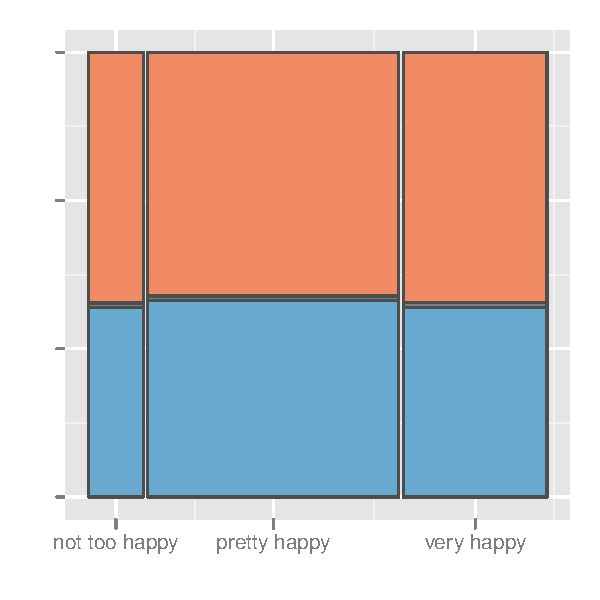
\includegraphics[width=0.33\linewidth]{fact-happy-sex}%
  \includegraphics[width=0.33\linewidth]{fact-happy|sex}

  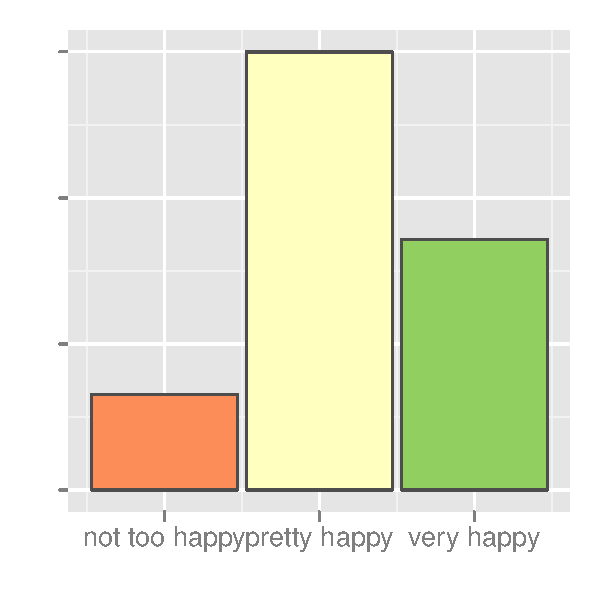
\includegraphics[width=0.33\linewidth]{fact-happy-2}%
  \includegraphics[width=0.33\linewidth]{fact-happy-sex-2}%
  \includegraphics[width=0.33\linewidth]{fact-happy|sex-2}

  \caption{Plots of the distribution of happiness and sex.}
  \label{fig:fact-simple}
\end{figure}


These techniques are also closely related to dimensional stacking \citep{leblanc:1990}

% Other papers to cite:
% 
% Generalised treemaps: \citep{vliegen:2006}
% Cocktailmaps: \citep{ahlberg:1996}
% Extension to mosaic: \citep{friendly:1999,hofmann:2000}
% Connection to models: \citep{theus:1999,hofmann:2001}


% Hierarchical coordinate systems 
%
% What are the common components of all these plots, and how can be describe
% them in a succinct way that also allows us to describe what tasks each
% display is good for?  We propose that there is one key feature that makes
% these plots special.  That is there their coordinate system, which is
% hierarchical.  
%
% In most coordinate systems that we are used to, such as Cartesian or polar
% coordinates, are symmetric in the sense that you can locate a point by
% starting from either dimension.  For example, in Cartesian coordinates you
% can identify either the x- or y-coordinate first, and the other next.  This
% also implies a distance symmetry when projected onto 2D Euclidean geometry.
% When you vary one coordinate by a small amount (holding all others constant)
% points in the projective geometry will be close.
%
% Neither of these properties hold for hierarchical coordinate systems. 
%
% We will discuss hierachical coordinate systems in general, and then present
% a specific hierachical coordinate system which gives rise to the area plots
% described previously. 

\section{Data}
\label{sec:data}

Two ways of representing data:

\begin{itemize}
  \item Multi-dimensional contingency table
  \item Data frame, with column of counts
\end{itemize}

The two are equivalent, but it's usually computational easier to work with the data frame version, because variables are explicit, and mathematically easier to work with the multidimensional array because multiplication is nicely defined.  Also deals better with sparsity and is common input to modelling algorithms.

Define the conditioning operator which makes the distribution uniform.  

In this paper, we'll use a small sample from the general social survey ({\sc gss}) focussing on happiness. 51\,020 observations from cross-section survey given yearly from 1972 to 2006.

\begin{itemize}
  \item Happy.  Discrete: ``very happy'', ``pretty happy'', ``not too happy''
  \item Age (in years), 18--89.
  \item Sex: ``female'', ``male''
  \item Degree: ``lt high school'', ``high school'', ``junior college'', ``bachelor'', ``gradudate''
  \item Relative financial status {\sf finrela}: ``far above average'', ``above average'', ``average'', ``below average'', ``far below average''
  \item Health: ``excellent'', ``good'', ``fair'', ``poor''
  \item Year: 1972--2006.
  \item Probability weight ({\sf wtsall}): 0.43--6.42.
\end{itemize}


\section{Display}
\label{sec:display}

Once we have made the decision to map area to proportion, then we need to impose some constraints on the set of possible tilings of the plane.  Some constraints are implied by our perceptual capabilities and others by simple geometry. (In general, we could also think of partitions of higher-dimensional spaces (e.g. 3d or 4d), but we will need to project these down to two for viewing anyway, so we might as well work directly in the final space.)

\begin{itemize}
  \item Area should be proportional to weight.  Imposed by problem statement.

  \item Rectangular partitions. It is easier to compare the areas of simple shape (i.e. rectangle vs polygon), and even better when one the length of one border is fixed, so we only need compare the length of the other \citep{cleveland:1984}.  Rectangular partitions are also recursive - a rectangular partition of a rectangular area produces rectangles.  There are a limited number of shapes that do this - triangles yes, circles, no.

  \item Containment / Non-overlapping.  To be able to see the complete area of each rectangle they must be non-overlapping, and each split must be nested within the shapes of the previous level.
  
\end{itemize}

Note, however, that each of these constraints can be profitably relaxed.  See Section~\ref{sec:relax} for details.

Let $a(i)$ give the area assigned to category $i$, which has proportion $f(i)$.  $a(i) \propto f(i)$ or $a(i) = k \dot a(i)$, and $a(i) = w(i) \times h(i)$ where $w$ and $h$ represent width and height respectively.  Most of the the partitions described below use additional constraints: $h(i) = \sqrt{k} f(i)^x$ and $w(i) = \sqrt{k} f(i)^y$ where $x + y = 1$.  This ensures that it is only necessary to inspect one border to compare magnitudes.

The other chief difference between different tiling methods is whether or not they are space filling.  Space filling methods will ensure that areas are larger, but typically make it harder to compare magnitudes because scales no longer align.

The following two sections discuss particular partitions of the plane based on either a 1d or 2d pmf.  Displays of higher dimensional pmfs must be made by recursive combinations of these.  

\subsection{1d primitives}

There are three 1d primitives, as displayed in Figure~\ref{fig:part-1d}:

\begin{itemize}
  \item {\bf bar}: height is proportional to value, width equally divides space. Bars allow comparison between absolute numbers, but are not space filling.  They occupy sum(values / max(values)) of the total area.  Bars can be arranged horizontally (``hbar'') or vertically (``vbar'').

  \item {\bf spine}: width is proportional to value, height equally divides space. Splines are space filling, but make it more difficult to compare absolute counts.  Splines can be arranged horizontally (``hspline''),  vertically (``vspline''), or can automatically pick their orientation (``spline'').

  \item {\bf treemap}: no restrictions on height and width. Comparing the areas is the most difficult perceptually, and are most useful when there are a large number of categories.  There are a many variations of the treemap; this paper uses the squarified treemap \citep{bruls:1999}.

\end{itemize}

\begin{figure}[htbp]
  \centering
    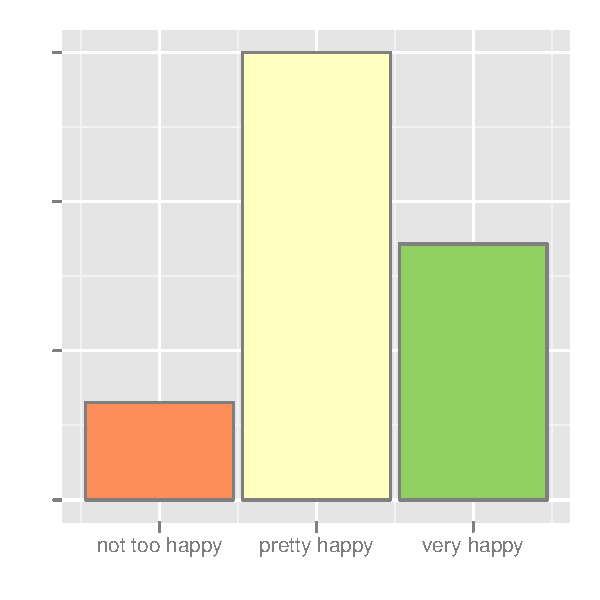
\includegraphics[width=0.33\linewidth]{part-hbar}%
    \includegraphics[width=0.33\linewidth]{part-hspline}
    % 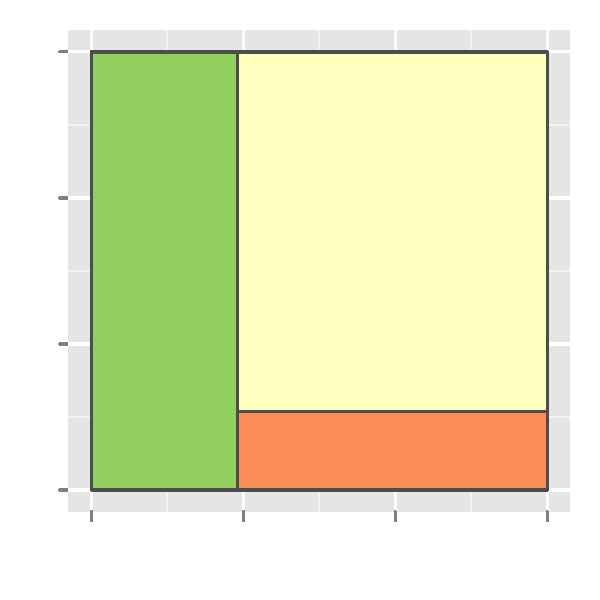
\includegraphics[width=0.25\linewidth]{part-treemap}

  \caption{1d partitions showing proportions 0.5, 0.2, 0.2 and 0.1. From left to right: horizontal bars, horizontal splines, and a treemap.}
  \label{fig:part-1d}
\end{figure}


\subsection{2d primitives}

\begin{itemize}
  \item {\bf fluct}: width and height proportional to square root of value. Flucts allow comparisons of absolute numbers in two directions. 
  
\end{itemize}

One special 2d case is the equal bin size plot - which all 1d x 1d primitives and the fluct collapse to when proportions are equal, as when conditioned.

Figure~\ref{fig:fluct} shows these two behaviours, looking at the relationship between happiness, health and financial status. On the left, a display of the raw proportion shows that most people are in good health and average financial standing, but it is difficult to see how happiness varies because the size of the squares is variable. On the right, conditioning on financial status and health makes all squares the same size and makes it easier to see the conditional distribution of happiness - people tend to be happier the healthier and the richer they are

\begin{figure}[htbp]
  \centering
    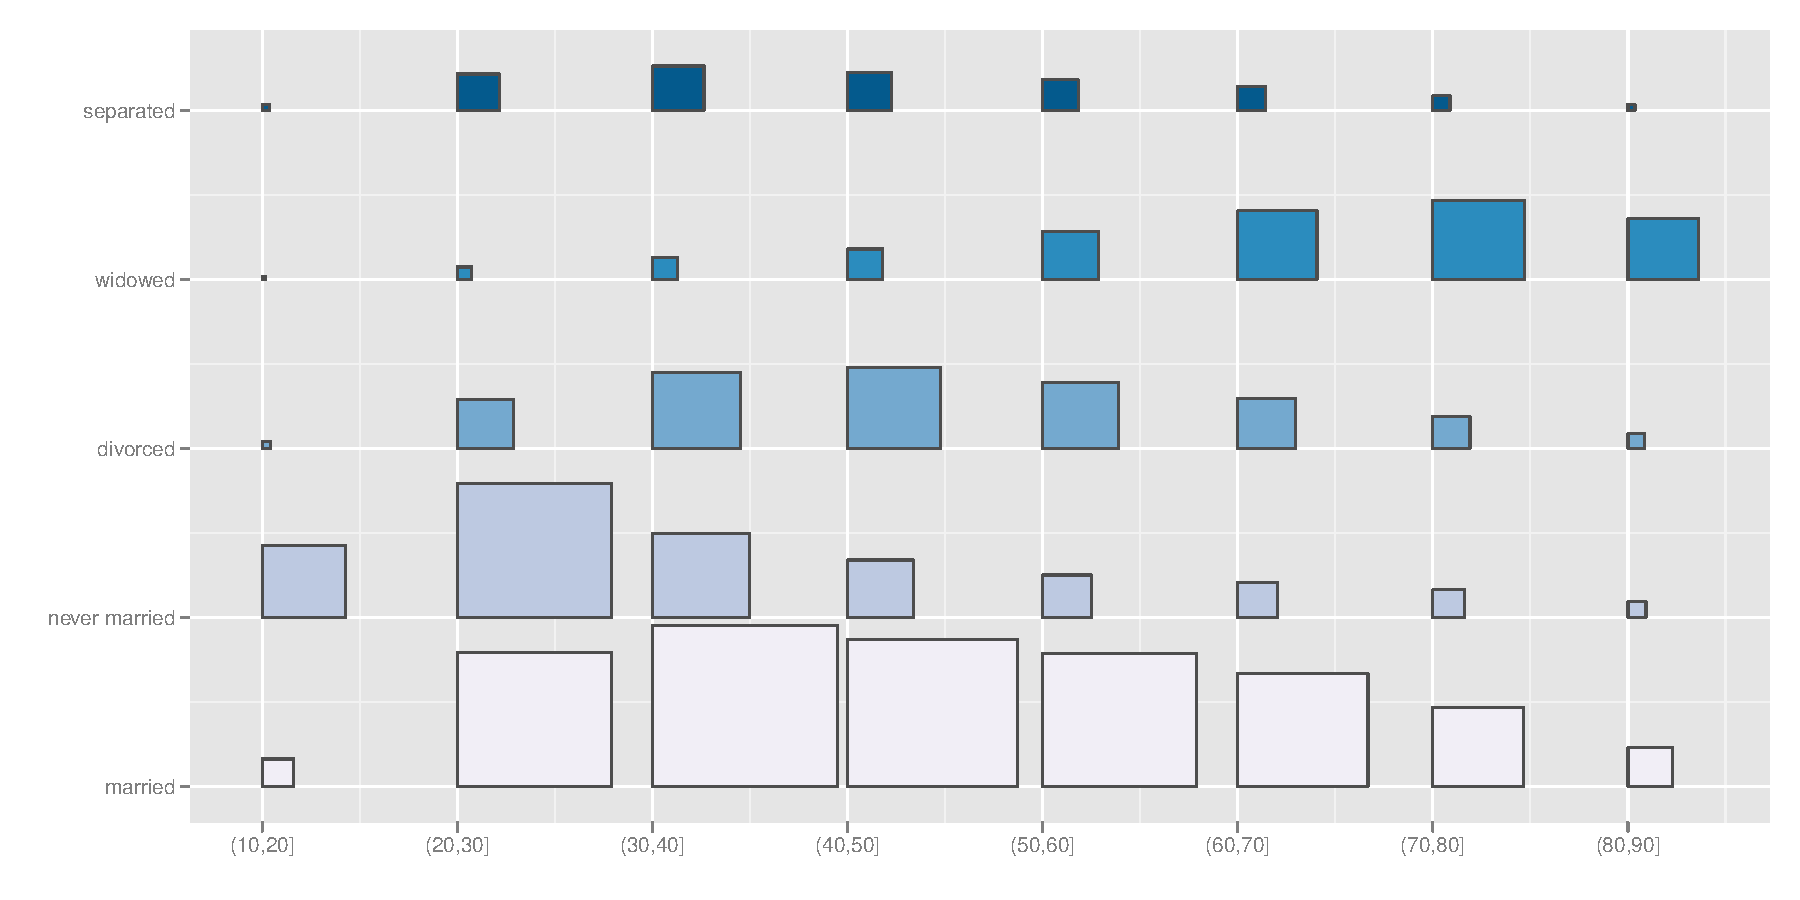
\includegraphics[width=0.5\linewidth]{part-fluct}%
    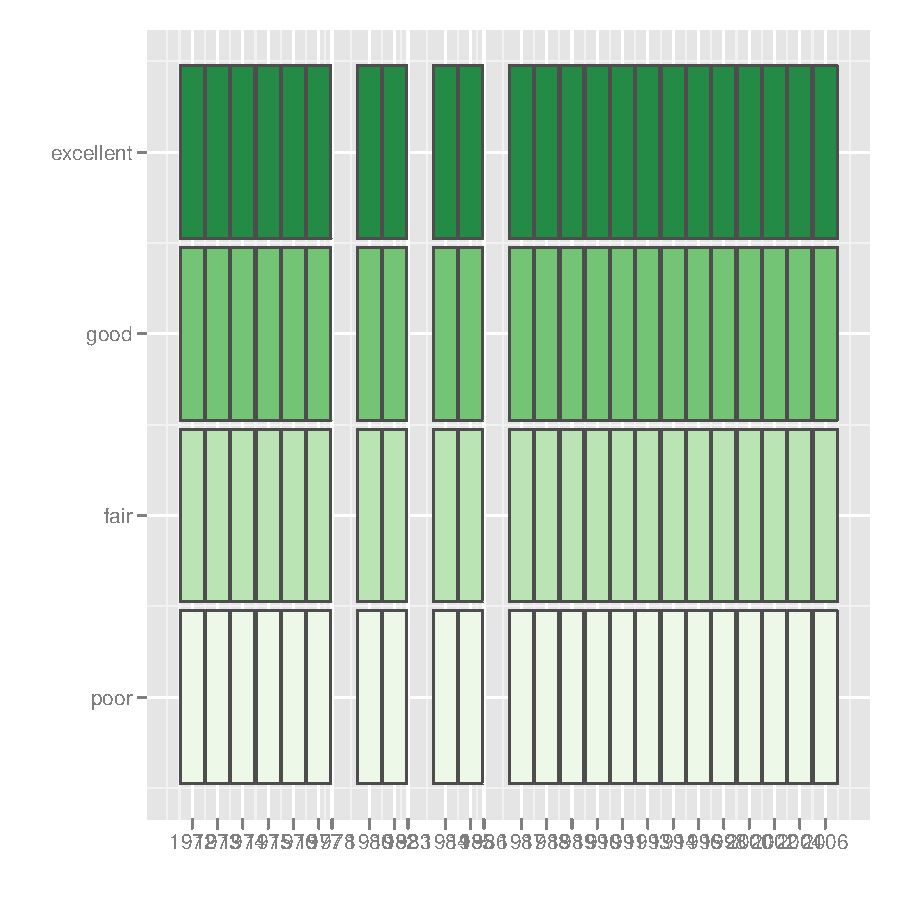
\includegraphics[width=0.5\linewidth]{part-fluct-cond}
  \caption{caption}
  \label{fig:fluct}
\end{figure}

\subsection{Plot templates}

The sequence of partitioning choices defines different named area plots:

\begin{itemize}
  \item {\bf Barchart} (1d). 1 hbar.
  \item {\bf Column chart} (1d). 1 vbar.
  \item {\bf Spineplot} (1d). 1 vspline.

  \item {\bf Stacked} barchart (2d). 1 hbar and 1 vspine.
  \item {\bf Nested} barchart (2d).  2 hbars. \citep{peltier:2009}
  \item {\bf Fluctuation} diagram (2d): fluct. 

  \item {\bf Equal bin size} plot (3d): fluct and vspline, provided the final two variables are uniform.

  \item {\bf Mosaic} plot (nd).  Alternating hspines and vspines.  \citep{hartigan:1984,hartigan:1981,friendly:1994,hofmann:2003}
  \item {\bf Double-decker} plot (nd).  $n-1$ hspines and 1 vspine. \citep{hofmann:2001}
  \item {\bf Treemap} (nd): n spines. \citep{shneiderman:1992}
  \item {\bf Squarified treemap} (nd): n squares. \citep{bruls:1999}
  
\end{itemize}

% http://peltiertech.com/Utility/ClusterStackUtility.html

\begin{itemize}
  
\end{itemize}

Trellis graphics are another type of display that uses categorical variables to create small multiples for different subsets of the data. Visually, trellis graphics look like equal-bin-size plots with another plot drawn inside each bin. 

\section{Relaxing constraints}
\label{sec:relax}

\subsection{Area not proportional to weight}

It can be useful to violate the constraint that area should be proportional to weight to distinguish between zeros and very small values.  A zero weight should have zero area, but giving it positive area can be useful so it's actually possible to see!  Similarly for very small values which would otherwise occupy less than a pixel, useful to constain to minimal perceptible size.

Antony's zooming, where you also truncate the maximum size.

Image.

\subsection{Levels not contained}

The cascaded treemaps of \citet{lu:2008} is an idea that illustrates how the violation of containment can be productive.  In the cascaded treemap, each level is slightly offset from the one above to create a pseudo-3d perspective.
This makes it easier to see all the levels of the hierarchy, not just the lowest level.

Example.

\subsection{Non-rectangular partitions}

Pie charts fall out naturally, as bars in polar coordinates, with angle and radius instead of height and width. And to ensure that counts stay proportional to areas, the square-root is taken of the y-axis. This is related to the infoslices of \citet{andrews:1998}, which only use half of the disk. Figure~\ref{fig:polar} illustrates a few product plots in polar coordinates.  Variables are happiness (top level in four categories) and sex (nested, two levels).

These displays generalise the fourfold displays of \citet{friendly:1995}. 

\begin{itemize}
  \item Pie charts
  \item Nightingale
  \item Bullseye chart 
\end{itemize}

\begin{figure}[htbp]
  \centering
    \includegraphics[width=0.25\linewidth]{hb-vb-cartesian}%
    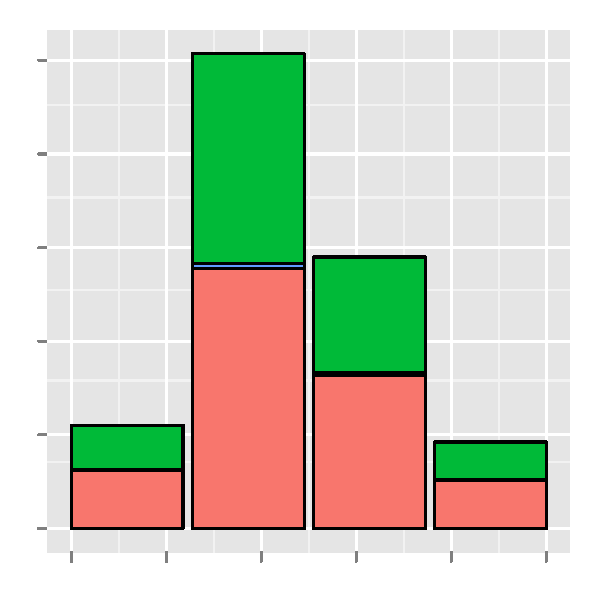
\includegraphics[width=0.25\linewidth]{hb-vs-cartesian}%
    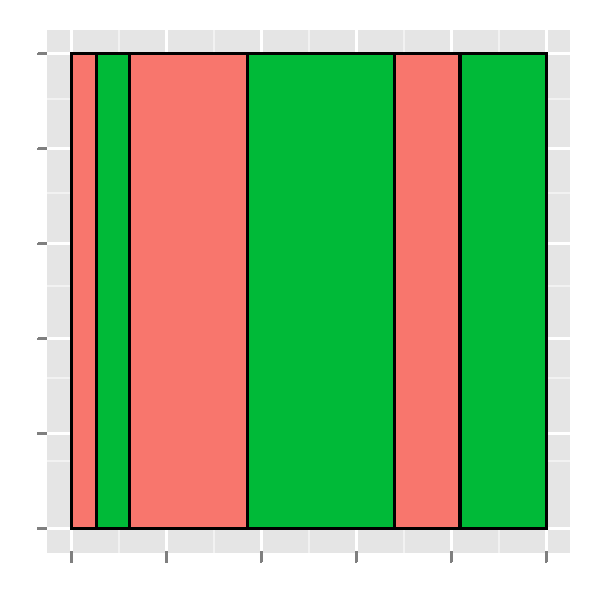
\includegraphics[width=0.25\linewidth]{hs-hs-cartesian}%
    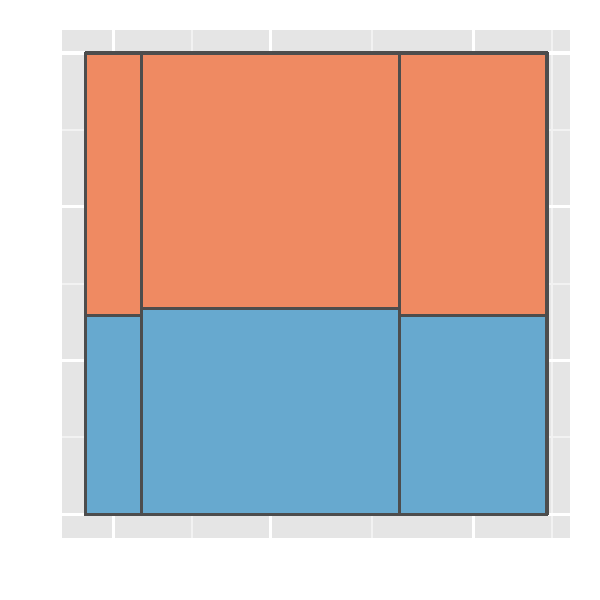
\includegraphics[width=0.25\linewidth]{hs-vs-cartesian}

    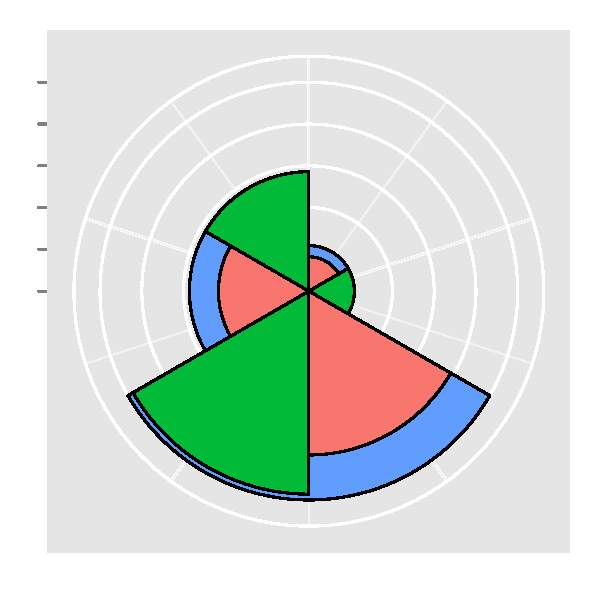
\includegraphics[width=0.25\linewidth]{hb-vb-polar}%
    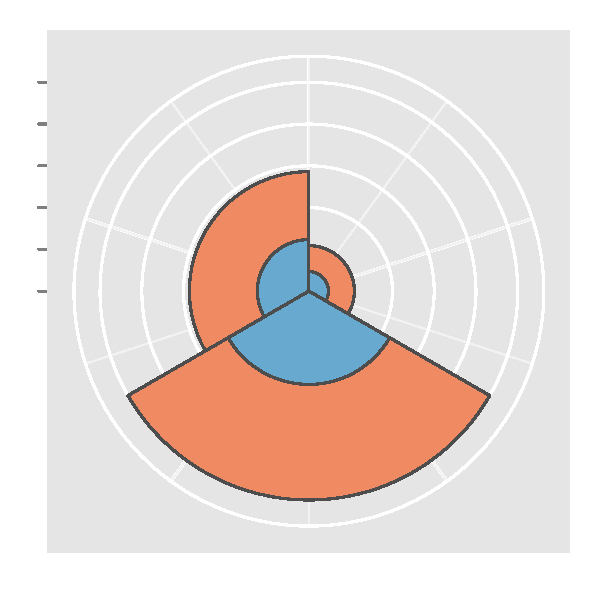
\includegraphics[width=0.25\linewidth]{hb-vs-polar}%
    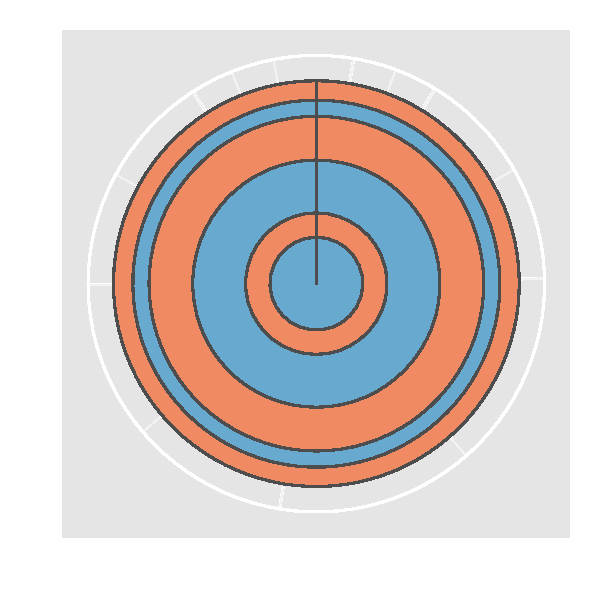
\includegraphics[width=0.25\linewidth]{hs-hs-polar}%
    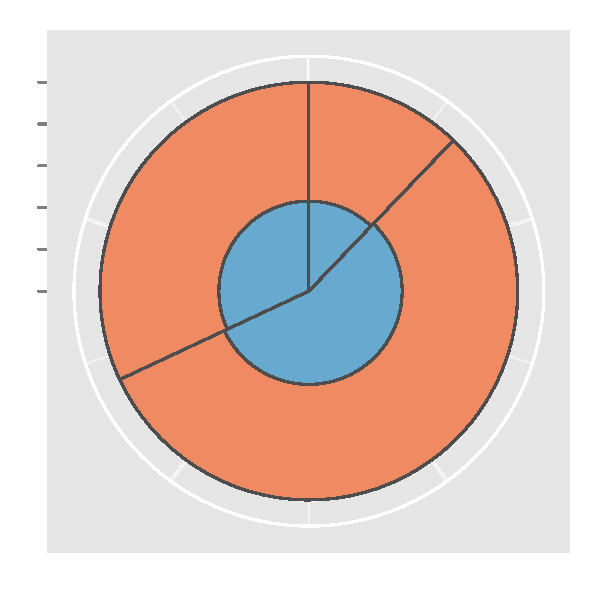
\includegraphics[width=0.25\linewidth]{hs-vs-polar}
  \caption{(Top) Area graphics in Cartesian coordinates.  (Bottom) Area graphics in polar coordinates.  From left to right: horizontal bar nested inside horizontal bar, vertical spline nested inside horizontal bar (stacked bar chart), horizontal spline nested in horizontal spline, horizontal spline nested in vertical spline (mosaic plot).}
  \label{fig:polar}
\end{figure}

Circular treemaps of \citet{wetzel:2008} which use circles instead of rectangles, but is not space filling because you can not tile a circular region with circles. The radial displays of \citet{stasko:2000} deliberately keep the radius constant in order to relatively highlight the lower levels.  Similarly so does the fanlens of \citet{lou:2007}

Other non-rectangular treemaps have been proposed, such as the space-filling curve approach of \citep{wattenberg:2005}, or the voronoi treemaps of \citep{wattenberg:2005}, but because of the perceptual difficultly of comparing areas of arbitrary polygons, these approaches tend to be attractive rather than useful.


% \section{Connection with log-linear models}


\section{Variations}
\label{sec:variations}

% Pseudo 2d, where you take a long 1d structure and wrap it into 2d.
% 
% Pseduo 1d, where you make a new variable from multiple variables.


\subsection{Weighting}
\label{sub:weighting}

We have assumed the probabilities represent counts, but without loss of generality we can use any set of non-negative, additive weights instead.  Some of the applications of such weighted plots are described in \citet{unwin:2007}.  Include a brief summary here.

\subsection{Continuous data}
\label{sub:continuous_data}

These techniques can also be used with continuous data, if the data is binned to create a categorical variable. This gives rise to the histogram and spinogram, analogues of the bar chart and spine chart respectively. A long standing tradition is that no gaps are displayed between adjacent rectangles when used for originally continuous data. Two examples are shown in Figure \ref{fig:cont-examples}.

\begin{figure}[htbp]
  \begin{center}
  \end{center}
  \caption{Area plots of originally continuous data}
  \label{fig:cont-examples}
\end{figure}

Give a few examples of non-traditional continuous-categorical plots.  Fluctuation diagram for exploring joint 2d distribution.  Mosaic for conditional.  Age and year distribution.  

Cat + continuous.

\subsection{Nested data}
\label{sub:nested_data}

We distinguish nested data from crossed data by the number of interactions with missing values.  Completely crossed data contains every combination of all variables.  Nested data contains 

Aka sparse vs. dense.

It is not always possible to determine nested data from inspection of the data alone, but may need knowledge of the data collection.  For example, if a survey of teachers within schools was performed, and each teacher was identified by a identifier unique within a school, it might look like the data was only missing a few combinations, when in fact it is meaningless.  

Or when you have a hierarchy.

Example dataset - Doug Bates teachers/schools?

Possibilities: create new variable which is interaction of nested vars, or drop missings/zeros.  Treemaps deal almost exclusively with nested data.

\section{Data analysis} % (fold)
\label{sec:data_analysis}

% section data_analysis (end)

\section{Labelling}
\label{sec:legends}

Labelling these plots is particularly challenging.  Future work!

\begin{itemize}
  \item Additional info 
  \begin{itemize}
    \item colour (map of the market)
    \item texture (sieve plots)
    \item photographs
    \item text (tables)
    \item embedded plots (time series in lab escape)
  \end{itemize}
  
  \item Display of hierarchy
  \begin{itemize}
    \item Spacing / borders
    \item Shading
    \item Cascading
    \item Labelling
  \end{itemize}
\end{itemize}

\section{Conclusions} % (fold)
\label{sec:conclusions}

% section conclusions (end)

% bibtool -x product-graphics -o references.bib
\bibliography{references}
\end{document}
